%calibrationPattern.tex
%Author: Russell Jackson September 2014

%This file is used to make stereo camera calibration patterns for use with mounting on lego bricks.
%The brick dimension were obtained from:
%//www.robertcailliau.eu/Lego/Dimensions/zMeasurements-en.xhtml

\documentclass[tikz,border=10mm]{standalone}
\usetikzlibrary{calc}

\def\xw{1}
\def\yw{9}
\def\rad{2.5mm}

\begin{document}
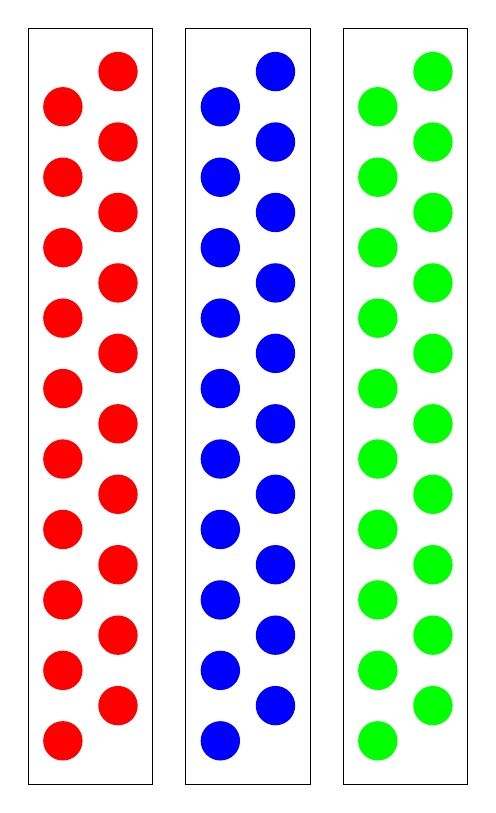
\begin{tikzpicture}[scale=1]

%table of lego widths w = 8.0mm*units-0.2mm
% 1 units wide:  7.8 mm                                                                                                                                  
% 2 units wide: 15.8 mm
% 4 units wide: 31.8 mm 
% (etc)

%lego heights 
% 1 unit: 9.6 mm

%This is the front side (red)
\draw (0.0mm ,0.0mm) rectangle (15.8mm,96mm);


\foreach \b in {0,...,\xw}{
    \foreach \c in {0,...,\yw}{

        \fill[red] (\b*7.0mm+4.4mm,\c*8.947mm+5.5mm+\b*4.47mm) circle [radius=\rad] ;

    }
}

%This is the right side (blue)
\draw (20.0mm ,0.0mm) rectangle (35.8mm,96mm);


\foreach \b in {0,...,\xw}{
	\foreach \c in {0,...,\yw}{
	% mod() must be used in order to calculate the right angle.
    % otherwise, when \b is greater than 28 the angle is greater
    % than 16384 and an error is raised ('Dimension too large').
   	% -- thx Tonio for this one.
    	%\pgfmathsetmacro{\angle}{mod(\goldenRatio * \b, 2) * 180}

    	%\pgfmathsetmacro{\sratio}{\b / \nbrcircles}
    	%\pgfmathsetmacro{\smArea}{\minArea + \sratio * \midArea}
    	%\pgfmathsetmacro{\smRadius}{sqrt(\smArea / pi) / 2 * \fudge}
    	%\addtocounter{cumulArea}{\smArea};
		%\pgfmathparse{sqrt(\value{cumulArea} / pi) / 2}
    	\fill[blue] (\b*7.0mm+4.4mm+20mm,\c*8.947mm+5.5mm+4.47mm*\b) circle [radius=\rad] ;
	}
}

%The left side is green
\draw (40.0mm ,0.0mm) rectangle (55.8mm,96mm);


\foreach \b in {0,...,\xw}{
	\foreach \c in {0,...,\yw}{
	% mod() must be used in order to calculate the right angle.
    % otherwise, when \b is greater than 28 the angle is greater
    % than 16384 and an error is raised ('Dimension too large').
   	% -- thx Tonio for this one.
    	%\pgfmathsetmacro{\angle}{mod(\goldenRatio * \b, 2) * 180}

    	%\pgfmathsetmacro{\sratio}{\b / \nbrcircles}
    	%\pgfmathsetmacro{\smArea}{\minArea + \sratio * \midArea}
    	%\pgfmathsetmacro{\smRadius}{sqrt(\smArea / pi) / 2 * \fudge}
    	%\addtocounter{cumulArea}{\smArea};
		%\pgfmathparse{sqrt(\value{cumulArea} / pi) / 2}
    	\fill[green] (\b*7.0mm+4.4mm+40mm,\c*8.947mm+5.5mm+4.47mm*\b) circle [radius=\rad] ;
	}
}

%\draw (0.0 mm, 136 mm) rectangle(50.0 mm 206.0 mm);

%\foreach 






\end{tikzpicture}
\end{document}
\geometry{letterpaper}
